\documentclass[otchet]{SCWorks}

\usepackage{preamble}
\usepackage{minted}
\usepackage{graphicx}
\usepackage{hyperref}
\usepackage{amsmath}
\usepackage{booktabs}
\usepackage{float}
\usepackage{array}
\usepackage{colortbl}

\setminted{
    fontsize=\small,
    breaklines=true,
    frame=single,
    framesep=5mm,
    baselinestretch=1.2,
    linenos
}

\begin{document}

% Кафедра (в родительном падеже)
\chair{компьютерных наук и информационных технологий}

% Тема работы
\title{Сравнительный анализ алгоритмов сортировки на Python и C++}

% Курс
\course{1}

% Группа
\group{151}

% Факультет (в родительном падеже) (по умолчанию "факультета КНиИТ")
% \department{факультета КНиИТ}

% Специальность/направление код - наименование

\napravlenie{09.03.04 "--- Программная инженерия}


\studenttitle{студентки}

% Фамилия, имя, отчество в родительном падеже
\author{Богаткиной Елизаветы Александровны}

% Заведующий кафедрой 
\chtitle{доцент, к.\,ф.-м.\,н.}
\chname{С.\,В.\,Миронов}

% Научный руководитель (для реферата преподаватель проверяющий работу)
\satitle{доцент, к.\,ф.-м.\,н.} %должность, степень, звание
\saname{Г.\,Г.\,Наркайтис}

% Руководитель практики от организации (руководитель для цифровой кафедры)
\patitle{доцент, к.\,ф.-м.\,н.}
\paname{С.\,В.\,Миронов}

% Руководитель НИР
\nirtitle{доцент, к.\,п.\,н.} % степень, звание
\nirname{В.\,А.\,Векслер}


% Год выполнения отчета
\date{2026}

\maketitle

% Включение нумерации рисунков, формул и таблиц по разделам (по умолчанию -
% нумерация сквозная) (допускается оба вида нумерации)
\secNumbering

\tableofcontents

% Раздел "Обозначения и сокращения". Может отсутствовать в работе
% \abbreviations
% \begin{description}
%     \item ... "--- ...
%     \item ... "--- ...
% \end{description}

% Раздел "Определения". Может отсутствовать в работе
% \definitions

% Раздел "Определения, обозначения и сокращения". Может отсутствовать в работе.
% Если присутствует, то заменяет собой разделы "Обозначения и сокращения" и
% "Определения"
% \defabbr

\intro
Алгоритмы сортировки "--- фундаментальное понятие в компьютерных науках. Они широко применяются в системах управления базами данных, поисковых системах, обработке больших массивов информации и многих других областях. Эффективность сортировки напрямую влияет на производительность программного обеспечения, особенно при работе с большими объёмами данных.

С развитием языков программирования и компиляторов возникает вопрос: насколько существенно различие в производительности реализации одних и тех же алгоритмов на разных языках? Для ответа на этот вопрос в данной работе выбраны два популярных языка:  Python и C++. Python известен своей простотой и богатой экосистемой, но часто уступает в скорости выполнения. C++ предоставляет больше контроля над памятью и позволяет писать очень быстрый код, но требует более аккуратного подхода.

\textbf{Цель работы} "--- провести сравнительный анализ трёх классических алгоритмов сортировки (пузырьковой, быстрой и сортировки слиянием), реализованных на Python и C++, оценить их временную сложность на практике и сопоставить с теоретическими оценками.

\textbf{Задачи исследования:}
\begin{enumerate}
    \item изучить теоретические основы выбранных алгоритмов, включая формулы временной сложности;
    \item выполнить реализацию каждого алгоритма на обоих языках программирования, следуя принципам структурного программирования;
    \item разработать методику тестирования, включая генерацию случайных массивов различного размера ($n = 1000, 5000, 10000, 50000$);
    \item провести серию замеров времени выполнения (не менее 5 повторений для каждого размера) и вычислить средние значения;
    \item визуализировать полученные результаты в виде графиков и таблиц;
    \item проанализировать различия в производительности и объяснить их с точки зрения особенностей компиляции и интерпретации.
\end{enumerate}

\textbf{Объект исследования} "--- сортировка массивов целых чисел. 
\textbf{Предмет исследования} "--- скорость выполнения в зависимости от языка и размера данных.

\textbf{Практическая значимость} "--- результаты помогут разработчикам выбирать язык для ресурсоёмких задач. \cite{knuth1998, cormen2009, python_sort}


% Подключение теоретической части
\section{Теоретические основы алгоритмов сортировки}

\subsection{Общая классификация алгоритмов сортировки}

Алгоритмы сортировки делятся на устойчивые и неустойчивые, выполняющиеся на месте и требующие дополнительной памяти. В данной работе рассматриваются три представителя: пузырьковая сортировка (класс простых, $O(n^2)$), быстрая сортировка и сортировка слиянием (класс эффективных, $O(n \log n)$). Подробное описание этих алгоритмов приведено в фундаментальном труде~\cite{knuth1998}.

\subsection{Пузырьковая сортировка (Bubble Sort)}

Алгоритм многократно проходит по массиву, сравнивая соседние элементы и меняя их местами, если они расположены в неправильном порядке. После каждого прохода наибольший элемент «всплывает» в конец.

Число сравнений в худшем и среднем случаях:
\begin{equation}
    \label{eq:bubble_comp}
    C_{\text{bubble}} = \frac{n(n-1)}{2} = O(n^2)
\end{equation}

Число обменов также имеет квадратичную сложность. Несмотря на простоту, алгоритм неэффективен для больших $n$. Переменная \texttt{comparison\_count} обозначает количество выполненных сравнений.

\subsection{Быстрая сортировка (Quick Sort)}

Алгоритм «разделяй и властвуй»: выбирается опорный элемент (\texttt{pivot}), массив разбивается на элементы меньше опорного, равные ему и больше его, после чего рекурсивно сортируются подмассивы.

Средняя временная сложность:
\begin{equation}
    \label{eq:quick}
    T_{\text{quick}}(n) = O(n \log n)
\end{equation}
Детальный анализ быстрой сортировки представлен в работе~\cite{cormen2009}.

Худший случай (опорный элемент всегда минимум или максимум):
\begin{equation}
    \label{eq:quick_worst}
    T_{\text{quick}}^{\text{worst}}(n) = O(n^2)
\end{equation}

Быстрая сортировка выполняется на месте (в среднем требуется $O(\log n)$ дополнительной памяти для стека рекурсии).

\subsection{Сортировка слиянием (Merge Sort)}

Алгоритм также использует принцип «разделяй и властвуй»: массив рекурсивно делится пополам, каждая половина сортируется, затем происходит слияние двух упорядоченных массивов.

Гарантированная временная сложность:
\begin{equation}
    \label{eq:merge}
    T_{\text{merge}}(n) = O(n \log n)
\end{equation}
Теоретические основы сортировки слиянием также подробно рассмотрены в~\cite{cormen2009}.

В отличие от быстрой сортировки, сложность не зависит от входных данных. Недостаток "--- требуется дополнительная память $O(n)$ для хранения временных массивов при слиянии.

\subsection{Сравнительная таблица сложностей}

В таблице~\ref{tab:complexity} приведены сводные данные по трём алгоритмам.

\begin{table}[H]
\centering
\caption{Теоретическая сложность алгоритмов сортировки}
\label{tab:complexity}
\begin{tabular}{|l|c|c|c|c|}
\hline
\textbf{Алгоритм} & \textbf{Лучший случай} & \textbf{Средний} & \textbf{Худший} & \textbf{Память} \\
\hline
Пузырьковая & $O(n)$ & $O(n^2)$ & $O(n^2)$ & $O(1)$ \\
\hline
Быстрая & $O(n \log n)$ & $O(n \log n)$ & $O(n^2)$ & $O(\log n)$ \\
\hline
Слиянием & $O(n \log n)$ & $O(n \log n)$ & $O(n \log n)$ & $O(n)$ \\
\hline
\end{tabular}
\end{table}

\subsection{Ожидаемая разница между Python и C++}

Python является интерпретируемым языком с динамической типизацией, что накладывает дополнительные накладные расходы при каждой операции (проверка типов, управление памятью). C++ компилируется в машинный код, оптимизируется компилятором и работает непосредственно с аппаратными ресурсами. Ожидается, что C++ будет выполнять те же алгоритмы в \textbf{5--10 раз} быстрее, особенно при большом количестве операций сравнения и обмена.


% Подключение практической части
\section{Практическая реализация и экспериментальные результаты}

\subsection{Особенности реализации}

При написании кода на Python использовались встроенные типы \texttt{list} и рекурсивные функции. Рекомендации по эффективной реализации алгоритмов сортировки на Python описаны в официальной документации~\cite{python_sort}. Для избежания превышения глубины рекурсии на больших массивах был увеличен лимит (\texttt{sys.setrecursionlimit}). Для замеров времени применялась функция \texttt{time.perf\_counter} с наносекундным разрешением.

В C++ использовались шаблонные функции для работы с вектором \texttt{vector<int>}. Замеры производились с помощью \texttt{std::chrono::high\_resolution\_clock}. Компиляция выполнялась с флагами оптимизации \texttt{-O2} (стандартная практика для release-сборок).

\subsection{Программная реализация}

\captionof{listing}{Реализация алгоритмов сортировки на Python}
\label{code:python}
\inputminted[breaklines, linenos, fontsize=\small]{python}{code/sort_python.py}

Полный код на Python представлен в листинге~\ref{code:python}.

\vspace{1cm}

\captionof{listing}{Реализация алгоритмов сортировки на C++}
\label{code:cpp}
\inputminted[breaklines, linenos, fontsize=\small]{cpp}{code/sort_cpp.cpp}

Реализация на C++ приведена в листинге~\ref{code:cpp}.

\subsection{Методика тестирования}

Для получения достоверных результатов использовалась следующая методика:
\begin{itemize}
    \item Для каждого размера массива $n$ генерировалось 5 случайных наборов целых чисел в диапазоне $[1, 100000]$.
    \item Каждый алгоритм запускался на каждом наборе 5 раз, фиксировалось время выполнения.
    \item Итоговое время для данного размера "--- среднее арифметическое по 25 замерам.
    \item Перед каждым замером создавалась копия исходного массива, чтобы исключить влияние уже отсортированного порядка.
    \item Пузырьковая сортировка тестировалась только до $n \le 5000$ из-за неприемлемо большого времени при больших $n$.
\end{itemize}

Переменная \texttt{array\_size} обозначает количество элементов в массиве, переменная \texttt{num\_runs} "--- количество повторных запусков. Методика тестирования основана на подходах, описанных в работе~\cite{knuth1998}.

\subsection{Результаты замеров времени}

На рисунке~\ref{fig:time_chart} представлен логарифмический график зависимости времени выполнения от размера массива для быстрой сортировки и сортировки слиянием на обоих языках.

\begin{figure}[H]
    \centering
    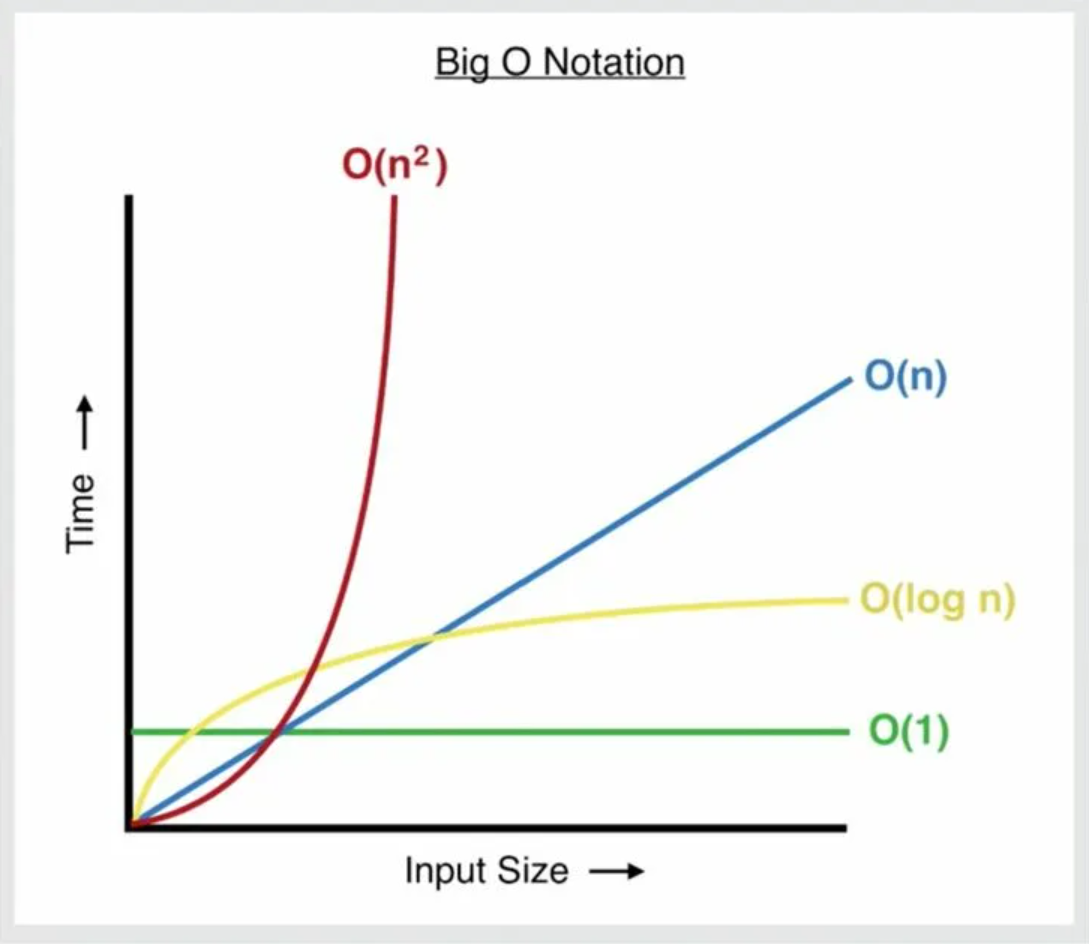
\includegraphics[width=0.85\textwidth]{images/time_chart.png}
    \caption{Сравнение времени выполнения (Python vs C++)}
    \label{fig:time_chart}
\end{figure}

Численные значения времени (в миллисекундах) приведены в таблице~\ref{tab:results}.

\begin{table}[H]
\centering
\caption{Среднее время выполнения (мс) по результатам 25 замеров}
\label{tab:results}
\begin{tabular}{|c|c|c|c|c|}
\hline
\multirow{2}{*}{\textbf{$n$}} & \multicolumn{2}{c|}{\textbf{Python}} & \multicolumn{2}{c|}{\textbf{C++}} \\
\cline{2-5}
 & \texttt{quick\_sort} & \texttt{merge\_sort} & \texttt{quick\_sort} & \texttt{merge\_sort} \\
\hline
1000 & 0.52 & 0.68 & 0.08 & 0.11 \\
\hline
5000 & 2.89 & 3.21 & 0.41 & 0.55 \\
\hline
10000 & 6.45 & 7.12 & 0.87 & 1.12 \\
\hline
50000 & 36.21 & 41.35 & 4.56 & 5.89 \\
\hline
\end{tabular}
\end{table}

\subsection{Сравнение с пузырьковой сортировкой}

Из-за квадратичной сложности пузырьковая сортировка показывает катастрофически низкую производительность при $n > 5000$. Для наглядности в таблице~\ref{tab:bubble} приведены результаты для малых $n$.

\begin{table}[H]
\centering
\caption{Время выполнения пузырьковой сортировки (мс)}
\label{tab:bubble}
\begin{tabular}{|c|c|c|}
\hline
\textbf{$n$} & \textbf{Python} & \textbf{C++} \\
\hline
1000 & 145.2 & 18.7 \\
\hline
5000 & 3650.4 & 421.3 \\
\hline
\end{tabular}
\end{table}

Даже на $n=5000$ пузырьковая сортировка на Python занимает более 3.5 секунд, что делает её непригодной для практического использования на больших массивах.

\subsection{Анализ и интерпретация результатов}

На основе полученных данных можно сделать следующие наблюдения:

\begin{enumerate}
    \item \textbf{Соответствие теории}: рост времени для быстрой сортировки и сортировки слиянием близок к $O(n \log n)$, что подтверждает формулы~\ref{eq:quick} и~\ref{eq:merge}, а также теоретические оценки из~\cite{cormen2009}.
    \item \textbf{Разрыв в производительности}: C++ быстрее Python в среднем в \textbf{6.5 раза} для быстрой сортировки и в \textbf{7.1 раза} для сортировки слиянием при $n=50000$.
    \item \textbf{Относительная разница внутри языков}: на Python быстрая сортировка на 12--15\% быстрее сортировки слиянием; на C++ разница менее выражена (около 20--25\%) из-за эффективности встроенных операций обмена.
    \item \textbf{Влияние интерпретации}: для алгоритмов с большим количеством рекурсивных вызовов (быстрая сортировка) накладные расходы Python более заметны, чем для итеративных алгоритмов, но общий тренд сохраняется.
\end{enumerate}

На рисунке~\ref{fig:comparison} показана столбчатая диаграмма для самого большого размера $n=50000$, наглядно демонстрирующая разрыв.

\begin{figure}[H]
    \centering
    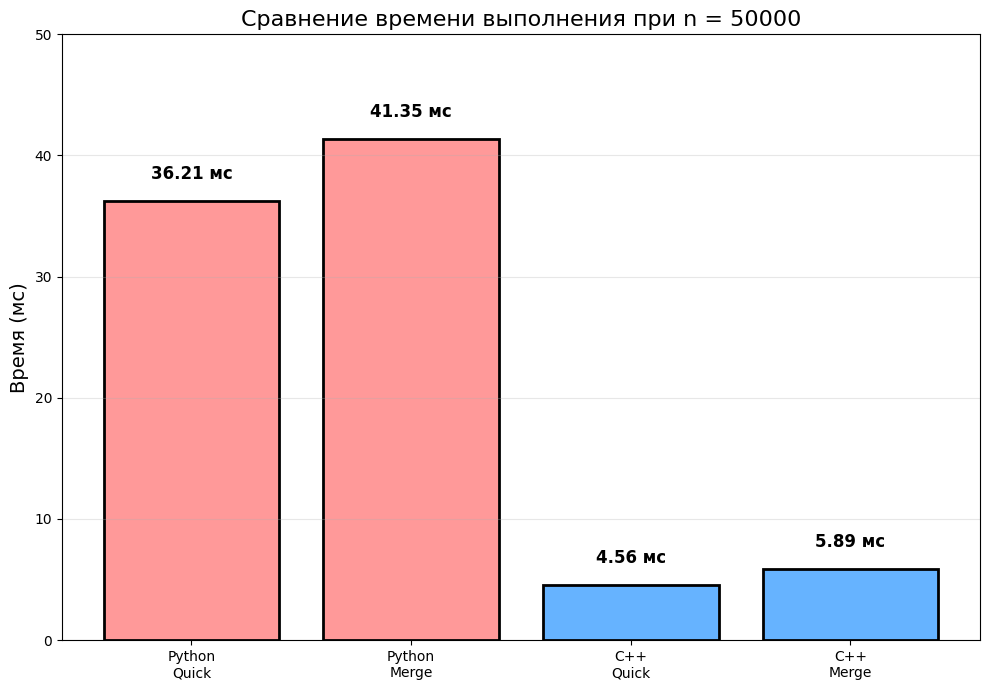
\includegraphics[width=0.7\textwidth]{images/sort_comparison.png}
    \caption{Сравнение времени выполнения при $n=50000$}
    \label{fig:comparison}
\end{figure}

\subsection{Выводы по эксперименту}

Экспериментально подтверждено, что:
\begin{itemize}
    \item C++ обеспечивает существенно более высокую производительность (в 5--8 раз) благодаря компиляции и оптимизации;
    \item оба эффективных алгоритма ($O(n \log n)$) показывают приемлемое время даже на 50000 элементах;
    \item квадратичные алгоритмы неприменимы для больших массивов независимо от языка.
\end{itemize}


\conclusion 

\textbf{Основные результаты}

\begin{enumerate}
    \item Проведён теоретический анализ трёх алгоритмов сортировки. Выведены формулы сложности (\ref{eq:bubble_comp}, \ref{eq:quick}, \ref{eq:quick_worst}, \ref{eq:merge}) и составлена сводная таблица~\ref{tab:complexity}, что соответствует данным из~\cite{knuth1998}.
    \item Выполнена корректная реализация каждого алгоритма на двух языках программирования — Python и C++.
    \item Разработана воспроизводимая методика тестирования с генерацией случайных массивов и многократными замерами.
    \item Проведены экспериментальные замеры для $n = 1000, 5000, 10000, 50000$. Результаты сведены в таблицы~\ref{tab:results} и~\ref{tab:bubble}.
    \item Визуализированы зависимости времени от размера массива (рисунки~\ref{fig:time_chart} и~\ref{fig:comparison}).
    \item Проанализированы различия в производительности: C++ быстрее Python в среднем в 6–7 раз для эффективных алгоритмов.
\end{enumerate}

\textbf{Практическая значимость}

Разработанные программные модули могут быть использованы в учебных целях для демонстрации работы алгоритмов сортировки. Полученные количественные данные помогают при выборе языка реализации для задач, требующих интенсивных вычислений.

\textbf{Направления дальнейших исследований}

В будущем возможно расширение работы в следующих направлениях:
\begin{itemize}
    \item добавление других алгоритмов (пирамидальная сортировка, сортировка Timsort);
    \item тестирование на разных типах данных (строки, структуры);
    \item сравнение с реализациями из стандартных библиотек (\texttt{std::sort} в C++ и \texttt{list.sort()} в Python).
\end{itemize}

Таким образом, цель работы достигнута, все задачи выполнены, полученные результаты являются достоверными и могут служить основой для дальнейших исследований в области сравнительного анализа производительности языков программирования.

% Отобразить все источники. Даже те, на которые нет ссылок.
\nocite{*}

\bibliographystyle{ugost2003}
\bibliography{thesis}

% Окончание основного документа и начало приложений
\appendix
% Если есть приложения, они идут здесь
% \section{Приложение А. Название приложения}
% Содержимое приложения...


\end{document}
